%\section{Introduction}

%NMT systems are well suited for any problem that can be formulated as mapping an input sequence to an output sequence \citep{sutskever2014sequence}.
Human languages are very diverse and are different from each other in many aspects. There are around 6000 - 8000 languages that are currently spoken in the world. This count varies based on the definition of a \textit{language} \citep{evans2009myth}. This diversity also creates a barrier in communication and interaction. Machine Translation is a promising field that can be used to overcome the human language barrier. With the recent technological advancements in communication, there is an increasing need for seamless communication and content assimilation across languages. 

Machine Translation (MT) is the process of translating text automatically from one natural language to another \citep{russell2002artificial}. The development of MT systems can be broadly classified into three: rule based approach, statistical approach, and neural network based approach. Starting from the 1980s until recently, Statistical Machine Translation (SMT) approaches like phrase-based translation models \citep{och2002statistical,koehn2003statistical} gave promising results and dominated the field of machine translation. They were widely adopted and used in most of the translation engines. 


Neural Machine Translation (NMT) is a recent approach to MT using neural networks.  \cite{kalchbrenner2013recurrent} proposed the first, successful end-to-end system using encoder-decoder architecture for MT. This led to rapid development of more complex encoder-decoder models by \cite{sutskever2014sequence,cho2014learning,bahdanau2014neural,vaswani2017attention}, each with additional functionality and improved performance. In the \textit{Conference on Machine Translation (WMT 2015)}, only one purely neural network based MT system was submitted, and it was outperformed by a statistical MT system. In the 2017 WMT conference, almost all the systems were NMT systems \citep{koehn2017neural}. As a result of this rapid development, popular translation engines like Google NMT, Microsoft Translator and Systran adopted NMT as a base technology for their translation system.

NMT requires a parallel corpus of source language and target language sentence pairs. These systems 
%, like other neural NLP systems, 
learn vector representation of the input words called \textit{word embeddings}. It is a way of representing words in a language using \textit{d-}dimensional \textit{word vector} $\vec{w} \in \mathbb{R}^{d}$. The word vectors capture essential information about the words such as semantics and morphology. In word vectors generated using continous bag of words(CBOW) models, a simple arithmetic on them can be used to answer analogies like \textit{man is to king as woman is to X} as shown below. 

\begin{align*}
\vec{man} - \vec{woman} + \vec{king} &  \approx \vec{queen} \\
\vec{walking} - \vec{walk} + \vec{stop} & \approx \vec{stopping}
\end{align*}



NMT systems will use the information captured in the word vectors and learn an input-output mapping, from a source language to the target language. The word vectors from the input sequence passed into a neural network are first mapped to a fixed length vector as shown in Figure \ref{enc_dec}. From this fixed length vector, the target language sentence is generated word by word. As words occur more often, they get semantically more accurate vector representations and are translated more accurately. %than the words that occur only a few times. 
Because of this, NMT requires a large training dataset to learn the mapping from an input (source) language to the output (target) language. 


\begin{figure}[ht]
	\centering
	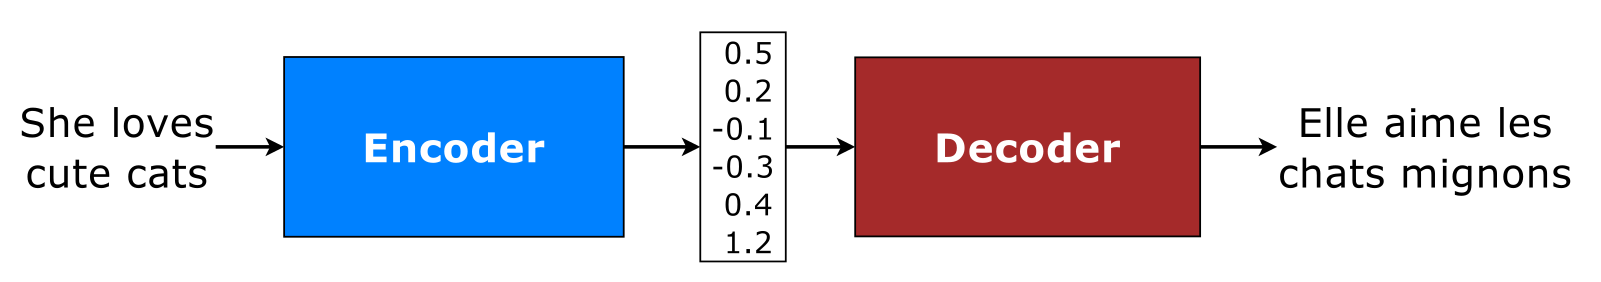
\includegraphics[scale=0.27]{images/enc_dec}
	\caption{General architecture of NMT systems. Figure taken from \cite{luong2016neural}}
	\label{enc_dec}
\end{figure}
%Because of this, common words are translated more accurately than rare and unknown words.

\section{Motivation}
%For example, these systems do not perform well  Another major challenge in NMT systems is their inability to handle large vocabulary\citep{koehn2017six}. 
Although NMT systems have shown promising results in the past few years, there are a number of challenges that these systems face. Some of the major challenges are: poor translation quality under low-resource conditions, poor translation of out-of-domain data, and inability to handle a large vocabulary \citep{koehn2017six}. These challenges are usually more pronounced in languages with rich morphology. 

\subsection{Morphologically rich, low-resource languages}
Morphologically rich languages such as Turkish, Tamil, German, Finnish etc., encode more information like gender, tense, number, etc. in a word as shown in Table \ref{turkish}. These languages also have a very large vocabulary since there can be large number of word forms per lexeme. Morphologically poor languages like English rely on word order (syntax) and context to convey this information. %In English, \textit{run, running, ran, runs} are all the forms of same lexeme \textit{run}.



\begin{table}[ht]
	\centering
	\resizebox{!}{4cm}{
	\begin{tabular}{@{}ll@{}}
		\toprule
		\textbf{Turkish}             & \textbf{English}                             \\ \midrule
		duy(-mak)                   & \textit{(to) sense}                          \\
		duygu                       & \textit{sensation}                           \\
		duygusal                    & \textit{sensitive}                           \\
		duygusallaş(-mak)           & \textit{(to) become sensitive}               \\
		duygusallaştırılmış         & \textit{the one who has been made sensitive} \\ 
		duygusallaştırılamamış      & \textit{the one who could not have been made sensitive} \\		
%		duygusallaştırılamamışlardan & \textit{from the ones who could not have been made sensitive} \\ \bottomrule
	\end{tabular}}
	\caption{Turkish - English Translation \citep{ataman2017linguistically} }
	\label{turkish}
\end{table}

Although benefits of NMT have been realized in high resource languages such as English and French, NMT is still a poor choice for languages, where parallel data for training is scarce. Neural methods learn poorly from low amount of data and hence, require a lot of data to perform well. 

\subsection{Research Problem}

The primary focus of this project is to improve the quality of machine translation for morphologically rich languages under low resource settings. NMT systems use a limited vocabulary, from 30,000 to 80,000 words, to control the computational complexity during training. While this vocabulary size is  large enough for languages like English, the performance of these models suffer in morphologically rich languages. To overcome this,  \cite{sennrich2015neural} proposed a system that can reduce the vocabulary size by splitting the words into common subwords. While this approach is sometimes sufficient, the words are not split at morphological boundaries.

Many inflected forms of words, as shown in Table \ref{turkish}, are usually scarce in the training dataset. Hence, the semantic and morphological information in the words is not captured in their word vectors. Addressing this problem can help us to improve the quality of machine translation for low-resource, morphologically rich languages.


In this project, we present a source language vocabulary expansion technique for handling a large vocabulary in NMT. This technique is particularly useful for low-resource, morphologically rich languages. The vocabulary is expanded based on morphological analysis of the Out of Vocabulary (OOV) words. For this purpose, we use a word embedding model based on sub-word units from \cite{bojanowski2016enriching}. To demonstrate the effectiveness of this approach, we present experimental evaluations on Turkish$\rightarrow$English and German$\rightarrow$English translation task. For comparison, we use global attention based NMT from \cite{luong2015effective} as a baseline.

%These systems are only as good as the data they are trained on. While English represents only 9\% of the world population, 54\% of the digital content is in English.
%This  Embedding models discussed in  \cite{bengio2003neural}, \cite{mikolov2013distributed}, \cite{pennington2014glove}, etc., learn word representations in continuous vector space where similar words occur closer to each other.  To get a good representation for each word the system has to be trained on large dataset of million of sentence. These word vector can also be trained on a large monolingual corpus and reused other tasks like machine learning.

%Another disadvantage of improving the vocabulary size, is that 


%The focus of this project will on the performance of NMT systems under low resource settings for morphologically rich languages.
%
%One of the challenges when using pre-trained word embeddings for any natural language processing (NLP) task is the issue of handling out-of-vocabulary (OOV) words. This problem occurs when a word that was unseen during training time occurs in testing phase during translation.  In this project, I propose and implement an NMT systems based on \cite{bahdanau2014neural} that is able to handle OOV words online during translation. OOV words will be analysed for their morphology and mapped to an in-vocabulary word using the technique from \cite{soricut2015unsupervised}.


%\subsubsection{Report outline}

\section{Report outline}

The project report is organized as follows. Chapter \ref{background} gives a background on recurrent neural networks and historical approaches for machine translation. In Chapter \ref{related}, related NMT systems that handle unknown words and their techniques are presented. In Chapter \ref{proposed}, we discuss our proposed vocabulary expansion technique and its architecture in detail. In Chapter \ref{comparision1}, we report on our comparison study of different techniques to handle OOV words. In Chapter \ref{experiments}, we present an evaluation of the proposed work on machine translation tasks for two language pairs. Finally, in Chapter \ref{conclusion}, we conclude the project report and provide future directions to extend the work carried out in this project.

%Dataset used in the project and evaluation metric are presented in Chapter \ref{experiments}. In the last section, the implementation status and timeline for the projects is given.
%
%a classic NMT model from \cite{bahdanau2014neural} and extending the work of \cite{soricut2015unsupervised} for handling OOV words online during translation. 


